% !TeX spellcheck = it_IT
%Cambio slide

\section{Wireless Personal Area Network WPAN}

\subsection{ISM Band}
Ci sono \textbf{porzioni di banda unlicensed}, ovvero che non necessitano di licenza per essere utilizzate. Sono riservate per usi industriali, scientifici e medici (ISM).\\

Bluetooth, Wi-Fi, apparecchi medici e tutti i dispositivi wireless comunicano sulle stesse frequenze. Essendo condiviso, le varie tecnologie devono tollerare interferenze.\\

\subsection{Pulse Code Modulation PCM}
Si tratta di una codifica lossless per onde. Partendo da un segnale continuo, l'ampiezza della curva viene quantizzata in livelli (intervalli) e viene effettuato un campionamento. La frequenza di campionamento è il doppio della frequenza massima da campionare (Teorema del campionamento di Shannon).

\begin{center}
	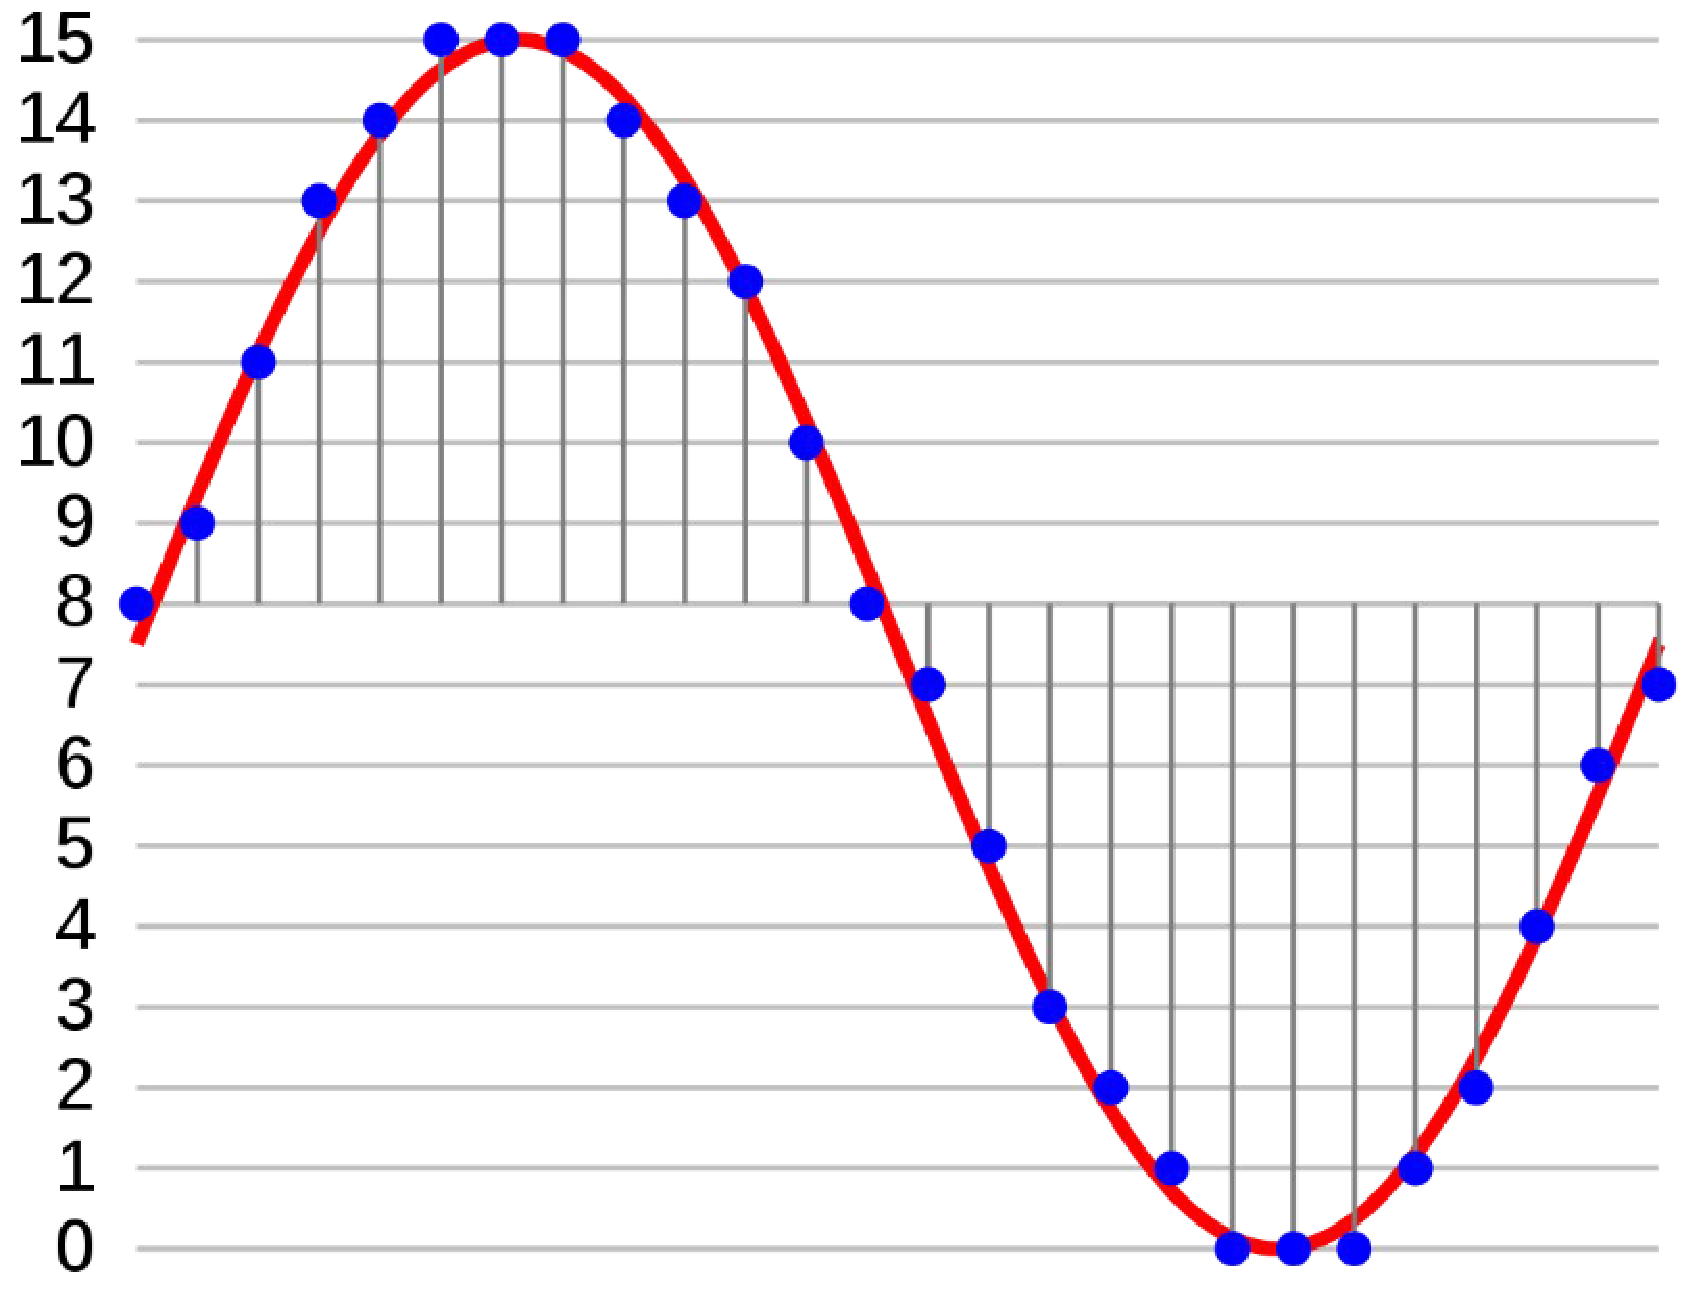
\includegraphics[width=0.7\linewidth]{img/wpan/PCM}
\end{center}

Per la voce telefonica: PCM 8bit $8000Hz$, quindi $64kbps$ (frequenza della voce $300 - 3400 Hz$). La musica viene campionata a 24bit $41/48kHz$.\\

\subsection{802.15.x}
Lo standard 802.15 comprende un insieme di tecnologie per la \textbf{comunicazione a corto raggio} (\texttt{\url{https://www.ieee802.org/15/}}).\\

Esempi di tecnologie: 
\begin{itemize}
	\item 802.15.1 Bluetooth
	\item 802.15.2 High-rate WPAN
	\item 802.15.4 Low-rate WPAN (es. Zigbee)
	\item 802.15.5 Mesh Networking (combinazione di High-rate e Low-Rate)
	\item 802.15.6 Body Area Network (BAN) pensato ad esempio per applicazioni in ambito medico
	\item 802.15.7 Visible Light Communication (VLC) (es. Vehicle-to-vehicle communication \& Li-Fi)
\end{itemize}

\subsection{Bluetooth}
Si tratta dello standard 812.15.1. Si compone di reti chiamate piconet ed all'interno della rete si ha un dispositivo \textbf{master} e \textbf{uno o più slave} sotto il controllo del master, che controlla la piconet.\\

\textbf{Caratteristiche}: 
\begin{itemize}
	\item Short range (10-50m nei casi d'uso tipici a seconda della classe di potenza del dispositivo, \texttt{\href{https://www.bluetooth.com/learn-about-bluetooth/key-attributes/range/\#estimator}{Bluetooth range estimator}})
	\item Usa la banda ISM $2.4GHz$
	\item Data Rate: $2.1 Mbps - 24Mbps$
\end{itemize}

Utilizzi: 
\begin{itemize}
	\item punto di accesso per dati e voce
	\item sostituzione di cavi (periferiche wireless)
	\item comunicazione ad hoc con altri dispositivi Bluetooth
\end{itemize}

\newpage

\subsubsection{Architettura dei protocolli} 
\begin{center}
	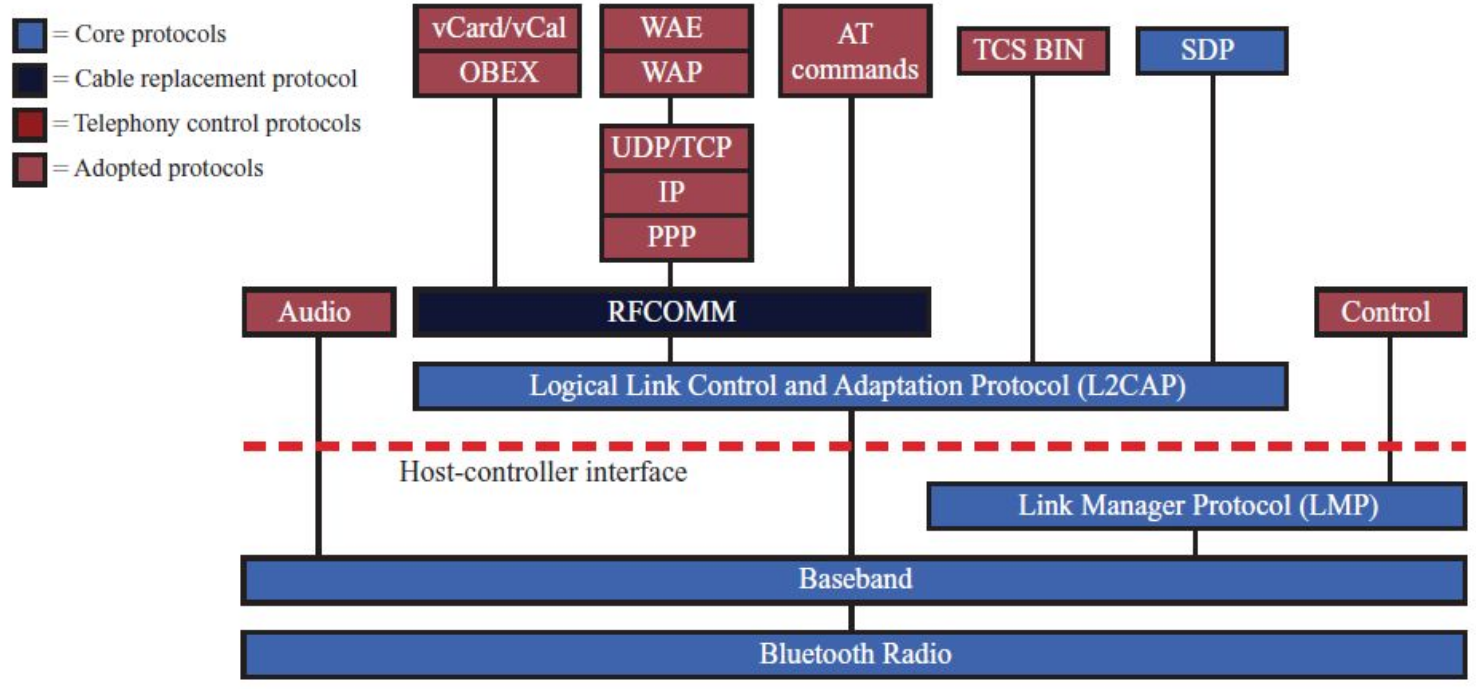
\includegraphics[width=0.95\linewidth]{img/wpan/archbt}
\end{center}
In blu sono i "core protocols", presenti in tutti i dispositivi Bluetooth. Gli altri (rossi e blu scuro) sono implementati solo se il dispositivo ne necessita, in base all'uso.\\

\paragraph{Bluetooth Radio:} La parte di livello fisico, specifica l'interfaccia radio: 
\begin{itemize}
	\item radio frequenze, quali frequenze utilizzare
	\item gestisce il frequency hopping
	\item decide lo schema di modulazioni in base al canale
	\item determina la potenza di trasmissione
\end{itemize}

\paragraph{Baseband:} Il livello di Baseband si occupa di 
\begin{itemize}
	\item stabilire la connessione con la piconet
	\item gestire l'indirizzamento
	\item formattazione dei pacchetti (frame)
	\item gestire le tempistiche di comunicazione (Time Division Duplex TDD e Time Division Multiple Access TDMA)
	\item gestisce la potenza di trasmissione (passa le indicazioni a livello radio)
\end{itemize}

\paragraph{Link Manager Protocol LMP:} Fa da "manager" del collegamento. Si occupa di:
\begin{itemize}
	\item configurare i collegamenti tra dispositivi
	\item gestione di collegamenti attivi
	\item funzionalità di sicurezza e cifratura
\end{itemize}
Si tratta di un protocollo di controllo, non passano dati ma gestisce il collegamento per i livelli sottostanti.

\paragraph{Logical Link Control and Adaptation Protocol (L2CAP):} I livelli precedenti erano implementati sul chip Bluetooth, da qui in su vengono implementati a livello software. Si occupa di:
\begin{itemize}
	\item adatta i protocolli di livello superiore al livello baseband
	\item astrarre tutto ciò che c'è sotto per i servizi a livelli superiori, \textit{Connectionless} e \textit{Connection-oriented}
\end{itemize}

\paragraph{Service Discovery Protocol SDP:} Gestisce le informazioni del dispositivo. Permette di comunicare
\begin{itemize}
	\item servizi disponibili sul dispositivo
	\item caratteristiche sul dispositivi
\end{itemize}
Stile architettura client-server: prevede interrogazioni richiesta-risposta per stabilire connessioni tra dispositivi Bluetooth.

\paragraph{Radio Frequency Communication RFCOMM:} Astrae il livello di Bluetooth, permette di "astrarre un cavo". Simula una comunicazione seriale e permette la trasmissione di dati tra dispositivi Bluetooth.

\paragraph{Livelli superiori:} I livelli in rosso sono protocolli "già esistenti", ciascun dispositivo può avere parte di questi protocolli in base all'uso, i livelli inferiori permettono la comunicazione a livello fisico.\\

\newpage

\paragraph{Profili:} Per avere determinate funzionalità un dispositivo deve seguire dei "profili". Esempi di profili:
\begin{center}
	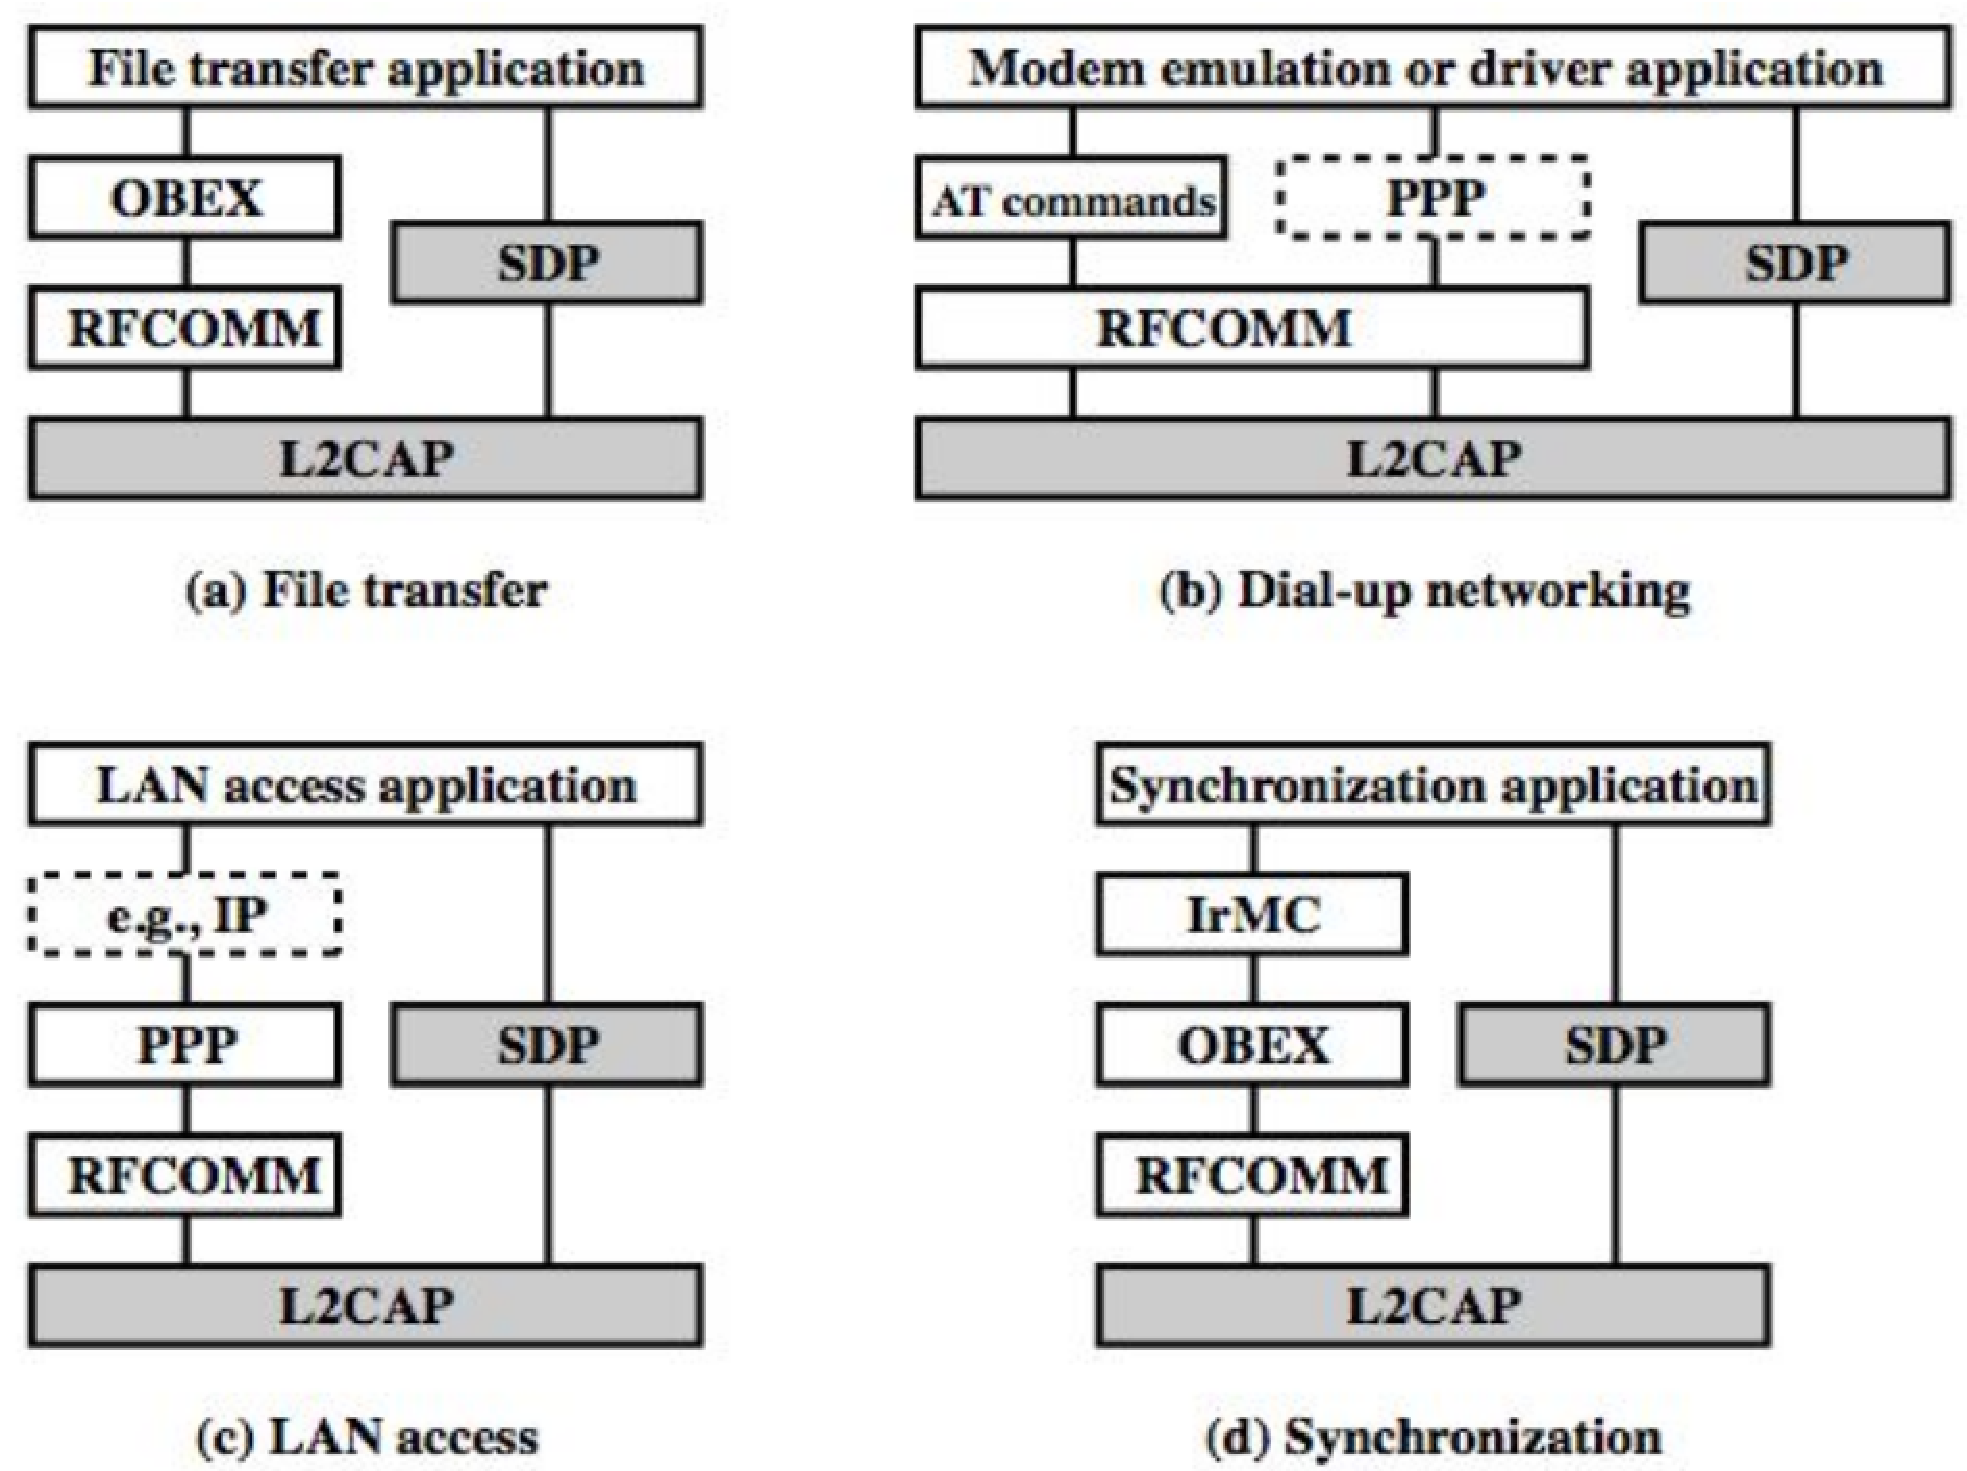
\includegraphics[width=0.7\linewidth]{img/wpan/profiles}
\end{center}
Questi sono standard, un dispositivo deve aderire ad uno o più profili (annunciati dal SDP) per avere il relativo utilizzo.\\

\newpage

\subsubsection{Piconet \& Scatternet}

\paragraph{Piconet:} Una piconet è composta da un \textbf{master} e 
\begin{itemize}
	\item \textbf{Active Slave (AS)}: membro attivo delle piconet, con un indirizzo Active Member Address (AMA) su 3 bit assegnato dal master (0 è il master, quindi 7 dispositivi al massimo)
	\item \textbf{Parked Slave (PS)}: membro della piconet ma temporaneamente disattivato, non possono comunicare attivamente ma solo ogni tanto tramite il Parked Member Address (PMA), 8 bit (0 è il master); un parked può tornare attivo solo se "c'è spazio"
	\item \textbf{Standby Slave (SS)}: non sconosciuti ma scollegati; non hanno indirizzi e possono quindi essere infiniti
\end{itemize}
\begin{center}
	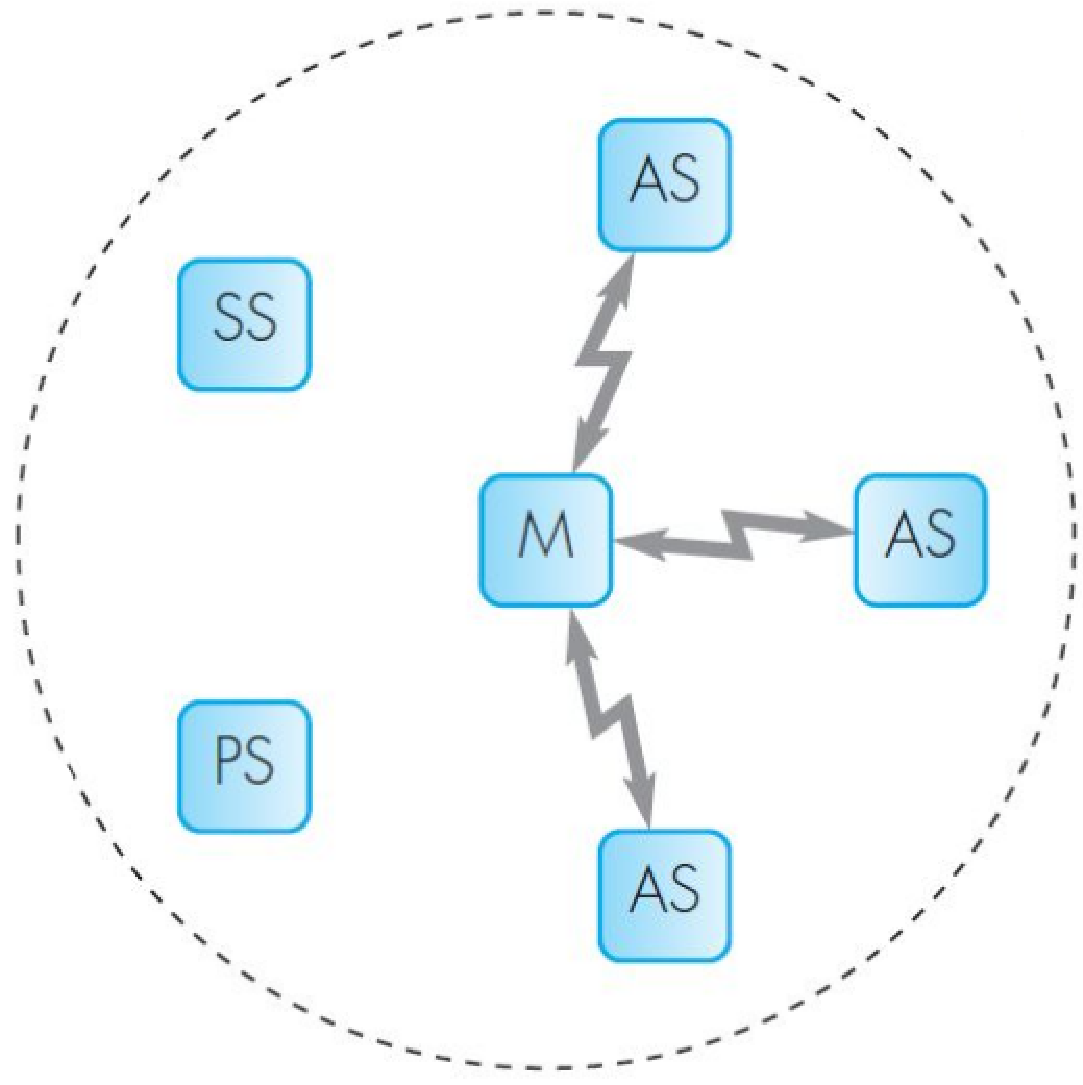
\includegraphics[width=0.35\linewidth]{img/wpan/pico1}
\end{center}

\paragraph{Scatternet:} La piconet ha al centro sempre un master, ma un dispositivo può appartenere a più piconet, portando ad una scatternet
\begin{center}
	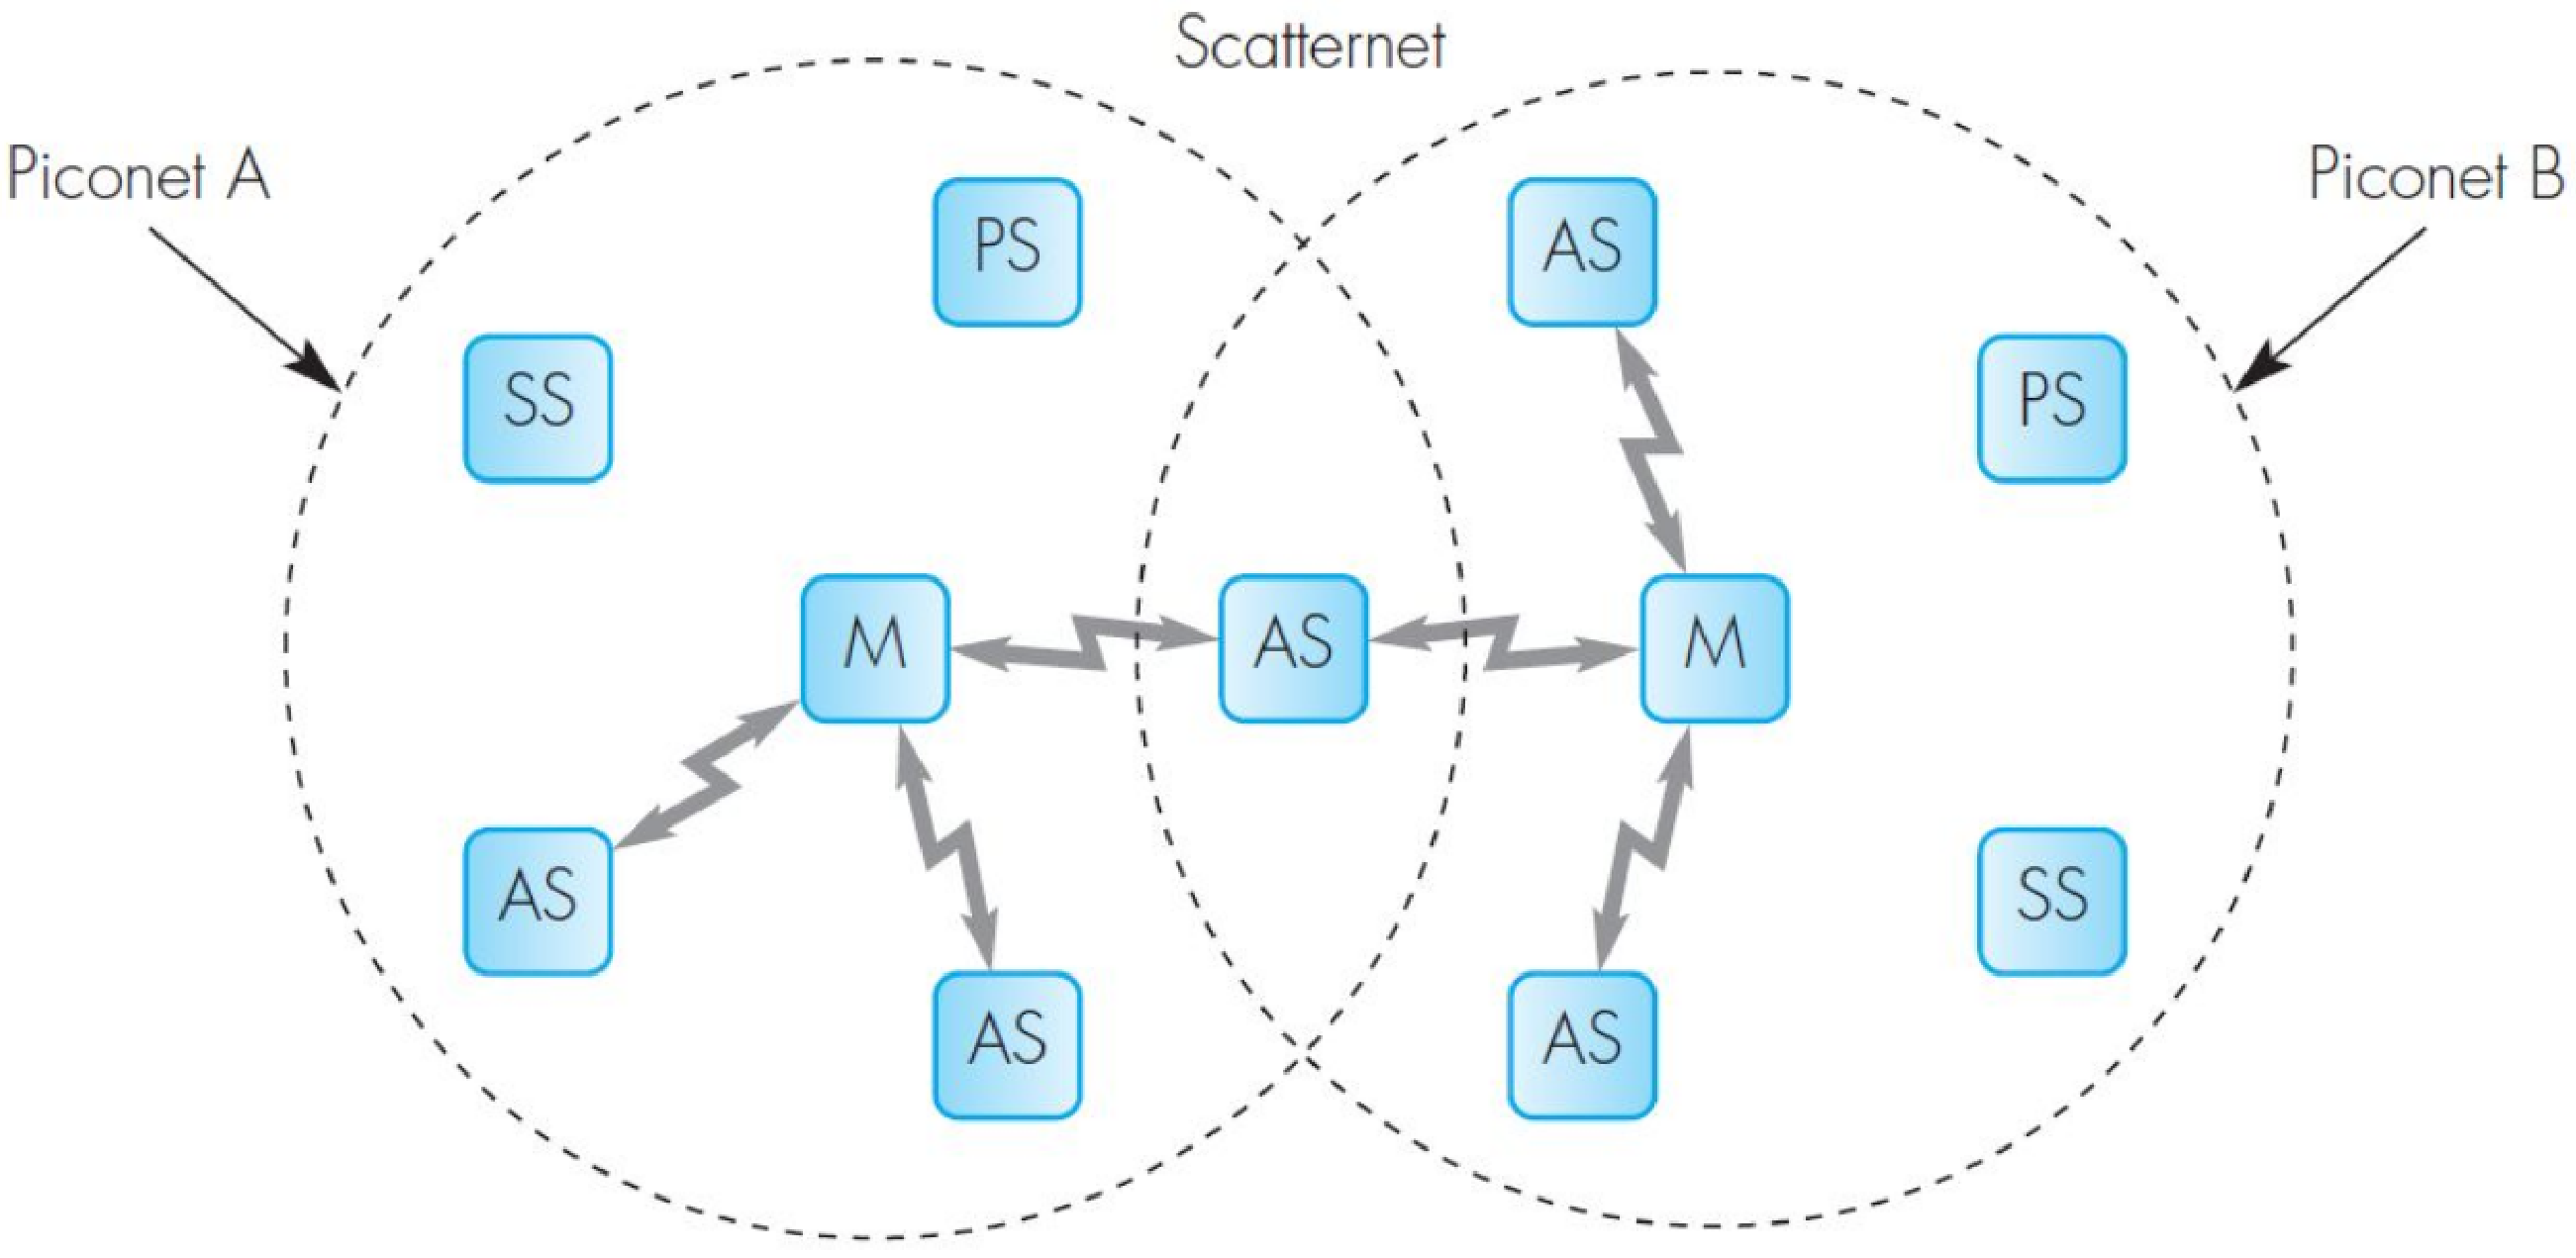
\includegraphics[width=0.7\linewidth]{img/wpan/scatter}
\end{center}
In qualsiasi caso i master lavorano in maniera completamente \textbf{separata}. Un AS attivo in due piconet diverse avrà indirizzamento diverso sulle due reti.

\subsubsection{Bluetooth Radio}
\paragraph{Specifiche radio Bluetooth 2.1:}
\begin{center}
	{
	\resizebox{0.98\textwidth}{!}{
	\renewcommand{\arraystretch}{1.2}
	\begin{tabular}{|l|l|l|}
		\hline
		& \textbf{Basic Rate (BR)} & \textbf{Enhanced Data Rate (EDR)} \\ 
		\hline
		\textbf{Topology} & \multicolumn{2}{c|}{Up to 7 simultaneous links in a logical star} \\ 
		\hline
		\textbf{Modulation} & GFSK & $\pi/4$-DQPSK and 8DPSK \\ 
		\hline
		\textbf{Peak data rate} & $1 Mbps$ & $2 Mbps$ and $3 Mbps$ \\ 
		\hline
		\textbf{RF bandwidth} & \multicolumn{2}{c|}{$220 kHz (-3 dB)$, $1 MHz (-20 dB)$} \\ 
		\hline
		\textbf{RF band} & \multicolumn{2}{c|}{$2.4 GHz$, ISM band} \\ 
		\hline
		\textbf{RF carriers} &  \multicolumn{2}{c|}{$23/79$}  \\ 
		\hline
		\textbf{Carrier spacing} &  \multicolumn{2}{c|}{$1MHz$}  \\ 
		\hline
		\textbf{Transmit power} &  \multicolumn{2}{c|}{$0.1W$}  \\ 
		\hline
		\textbf{Piconet access} &  \multicolumn{2}{c|}{FH-TDD-TDMA} \\ 
		\hline
		\textbf{Frequency hop rate} & \multicolumn{2}{c|}{1600 hops/s}\\ 
		\hline
		\textbf{Scatternet access} & \multicolumn{2}{c|}{FH-CDMA} \\ 
		\hline
	\end{tabular}}
	}
\end{center}
Per gestire le scatternet si usa FH-CDMA, anche in caso due scatternet comunichino sulla stessa frequenza si usa CDMA per poter distinguere i segnali.\\

\paragraph{Classi di potenza:} I dispositivi Bluetooth si differenziano in base alla classe di potenza
\begin{itemize}
	\item Power class 1: $100 mW$ 100 metri (senza ostacoli)
	\item Power class 2: $2.5 mW$ 10 metri (più tipico per BT)
	\item Power class 3: $1 mW$ 1-2 metri
\end{itemize}

\newpage

\paragraph{Comunicazione nelle piconet:} All'interno di una piconet vengono usate
\begin{itemize}
	\item Frequency Hopping FH: la frequenza è decisa dal master e condivisa agli slave nella piconet
	\item Time Division Duplex TDD: la comunicazione tra master e slave è gestita in tempo e alternata, prima comunica il master con lo slave, poi si invertono, con slot di $625\mu s$ (inclusa una guardia di $220 \mu s$)
	\item Time Division Multiple Access TDMA: per gestire più dispositivi nello stesso momento
\end{itemize}
\begin{center}
	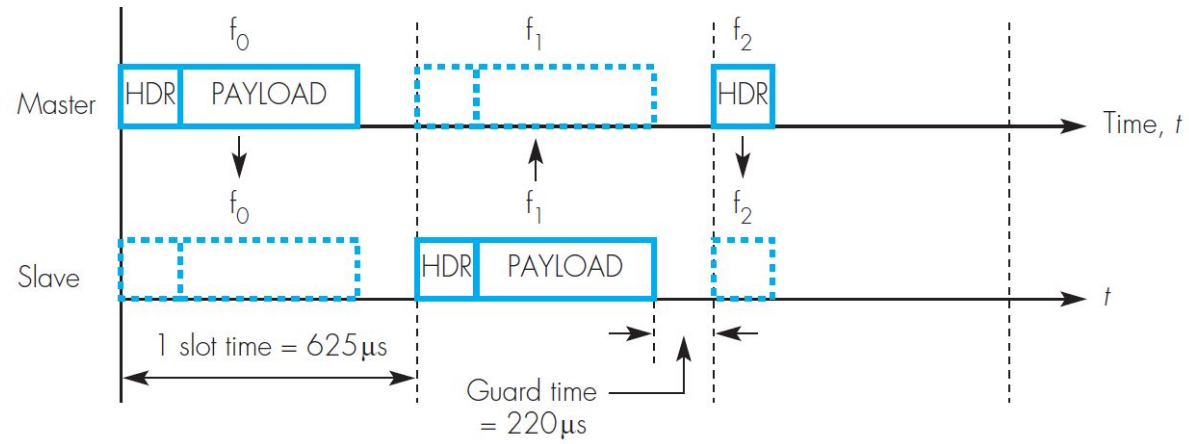
\includegraphics[width=0.9\linewidth]{img/wpan/picocomm}
\end{center}

%End L5

Esempio a più dispositivi: 
\begin{center}
	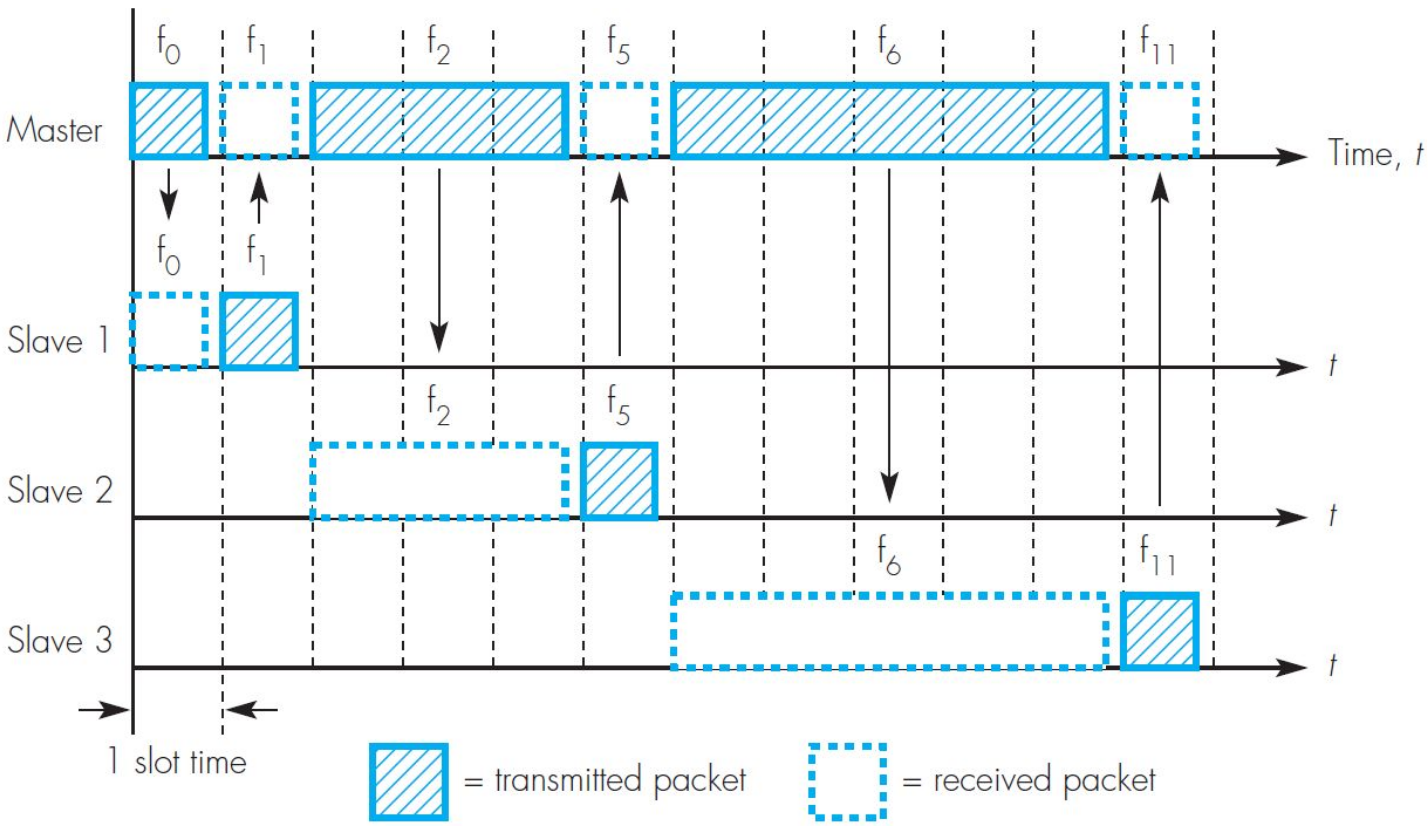
\includegraphics[width=0.9\linewidth]{img/wpan/picocomm2}
\end{center}

Nelle frequenze pari master a slave, nelle frequenze dispari viceversa. Più slave vengono coordinati tramite TDMA, ovvero il master decide chi parla in quale slot di tempo. La \textbf{dimensione dei messaggi} può essere di 1, 3 o 5 slot di tempo consecutivi (dispari per mantenere l'alternanza in TDD). Nell'header di ogni pacchetto c'è la dimensione.\\

La frequenza usata dal frequency hopping è data dal numero di timeslot passati, non dal numero di messaggi, quindi al time slot 5 viene usata la quinta frequenza $f_5$, anche se sono stati inviati solo 3 messaggi. Per una singola trasmissione (messaggio) viene mantenuta la stessa frequenza (non cambia a metà). All'interno della piconet tutti i clock devono essere sincronizzati.\\

\paragraph{Scatternet:} Nel caso di una scatternet, ogni piconet che la compone ha tutto diverso: diverse frequenze, diverso clock e di conseguenza completa autonomia. Un AS connesso a più piconet deve essere in grado di gestire le due connessioni indipendentemente.\\

Su 79 canali, cambiati ogni $625 \mu s$, può capitare una sovrapposizione (quindi interferenza), possibili soluzioni sono: 
\begin{itemize}
	\item FH su un numero ridotto di canali, e.g., ogni piconet su 20 canali e si spera non ci sia sovrapposizione in quei 20
	\item Si usa CDMA per evitare interferenze; il master comunica un codice ortogonale ai dispositivi all'interno della piconet (soluzione usata)
\end{itemize}

\newpage

\subsubsection{Baseband}

\paragraph{Tipologie di servizio:} Offre due possibili canali logici: 
\begin{itemize}
	\item \textbf{Synchronous Connection-Oriented Link (SCO)} point-to-point:
	\begin{itemize}
		\item canale audio/voce di $64kbps$ bidirezionale
		\item il master riserva una coppia di slot adiacenti ad intervalli regolari
		\item previsti fino al massimo di 3 canali SCO attivi contemporaneamente
		\item traffico real time
	\end{itemize}
	Garantiscono un bit rate fisso, un canale riservato, usato per casistiche sensibili al delay (real time).
	
	\item \textbf{Asynchronous Connectionless Link (ACL)} point-to-multipoint:
	\begin{itemize}
		\item canali ACL occupano gli slot rimanenti
		\item traffico dati con ciascuno degli slave
		\item un solo ACL contemporaneo fra master e uno slave
		\item traffico best effort (nessuna garanzia di delay)
	\end{itemize}
	Bit rate non costante, permette una qualità maggiore ma senza nessuna garanzia.
\end{itemize}
\begin{center}
	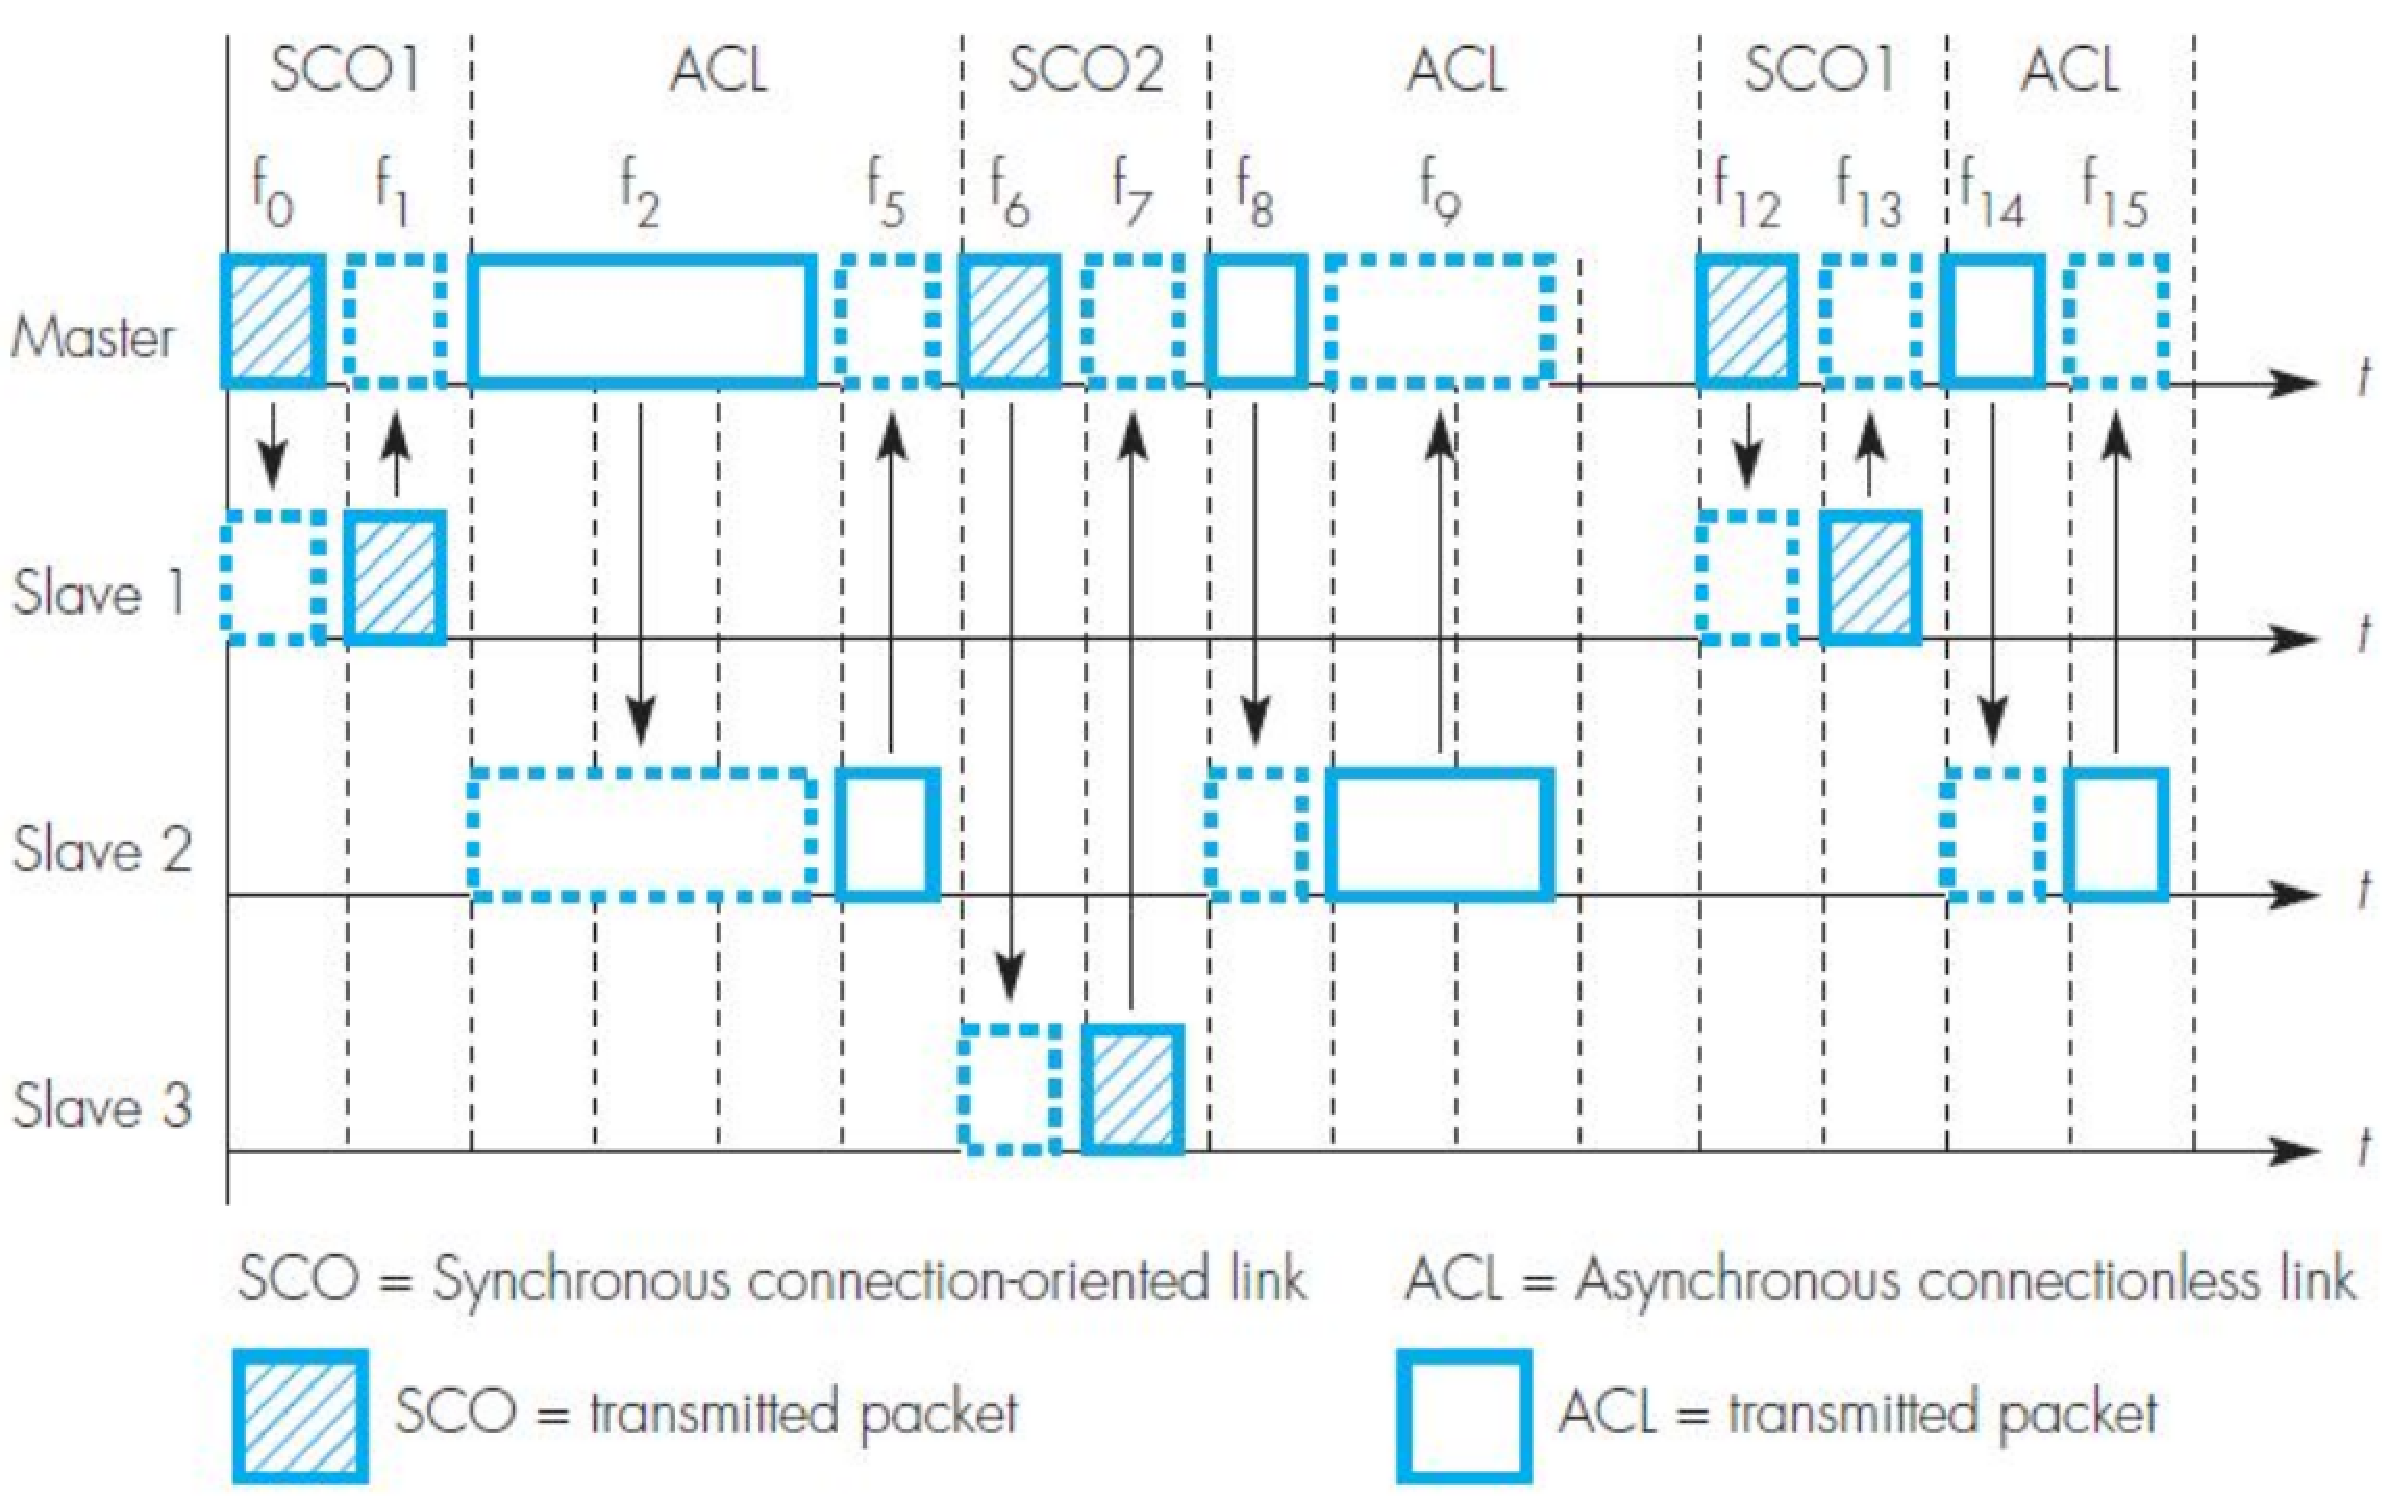
\includegraphics[width=0.9\linewidth]{img/wpan/scoacl}
\end{center}

\paragraph{Formato pacchetti:} 
\begin{center}
	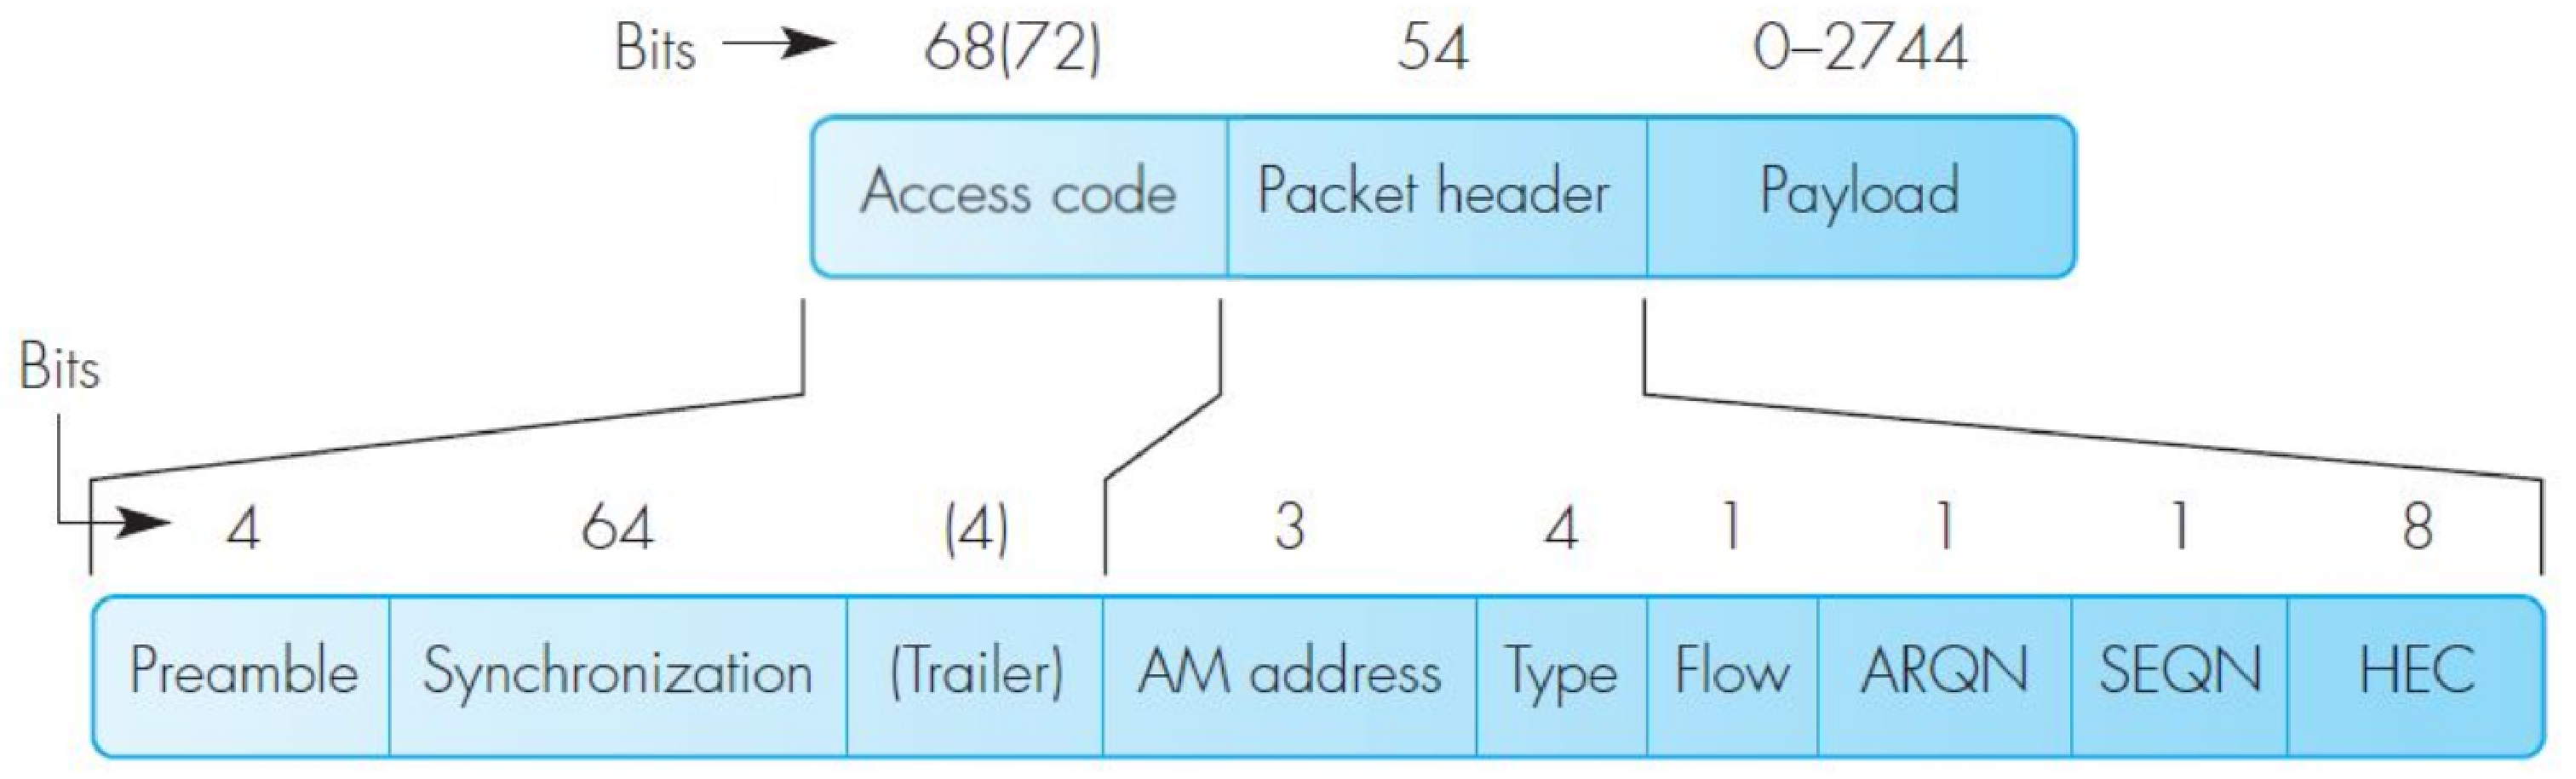
\includegraphics[width=0.9\linewidth]{img/wpan/basebandpacket}
\end{center}
Access code: utilizzato per sincronizzazione e identificazione. Può essere di 3 tipi:
\begin{itemize}
	\item Channel Access Code (CAC): identifica la piconet (derivato dai 48 bit dell'indirizzo hardware del master)
	\item Device Address Code (DAC): derivato dall'indirizzo hardware dello slave ed è usato dal master per chiamare il dispositivo (paging)
	\item Inquiry Address Code (IAC): usato per trovare l'indirizzo di un dispositivo vicino (durante la fase di inquiry)
\end{itemize}

Packet Header: ha diversi campi: 
\begin{center}
	    \begin{tabular}{|l|p{10cm}|}
		\hline
		\textbf{Campo Header} & \\ \hline
		AMA & Indirizzo del membro attivo della piconet \\ \hline
		Type & Identifica la tipologia del pacchetto e il formato del pacchetto SCO/ACL, numero di slot ecc... \\ \hline
		Flow & Per gli ACL: stop (1), resume (0) \\ \hline
		ARQN & 1 ACK, 0 NACK \\ \hline
		SEQN & Sequence number modulo 2 \\ \hline
		HEC & Controllo errori del campo header (1/3 FEC) \\ \hline
	\end{tabular}
\end{center}
ARQN e SEQN sono 2 bit necessari e sufficienti per il controllo degli errori (bastano grazie alla rigida struttura di comunicazione delineala al livello precedente).\\

%TODO Wtf, idk
Payload: contenuto effettivo del pacchetto può essere: 
\begin{itemize}
	\item SCO: 30 byte,  (FEC 0, 2/3, 1/3), che porta a massimo $64kbps$, dato che $(30 \cdot 8) \cdot (1600/6)$, ovvero $30 \cdot 8$ bit, 
	\item ACL: variabile da 0 a 343 byte
\end{itemize}

\paragraph{Controllo degli errori: }
\begin{center}
	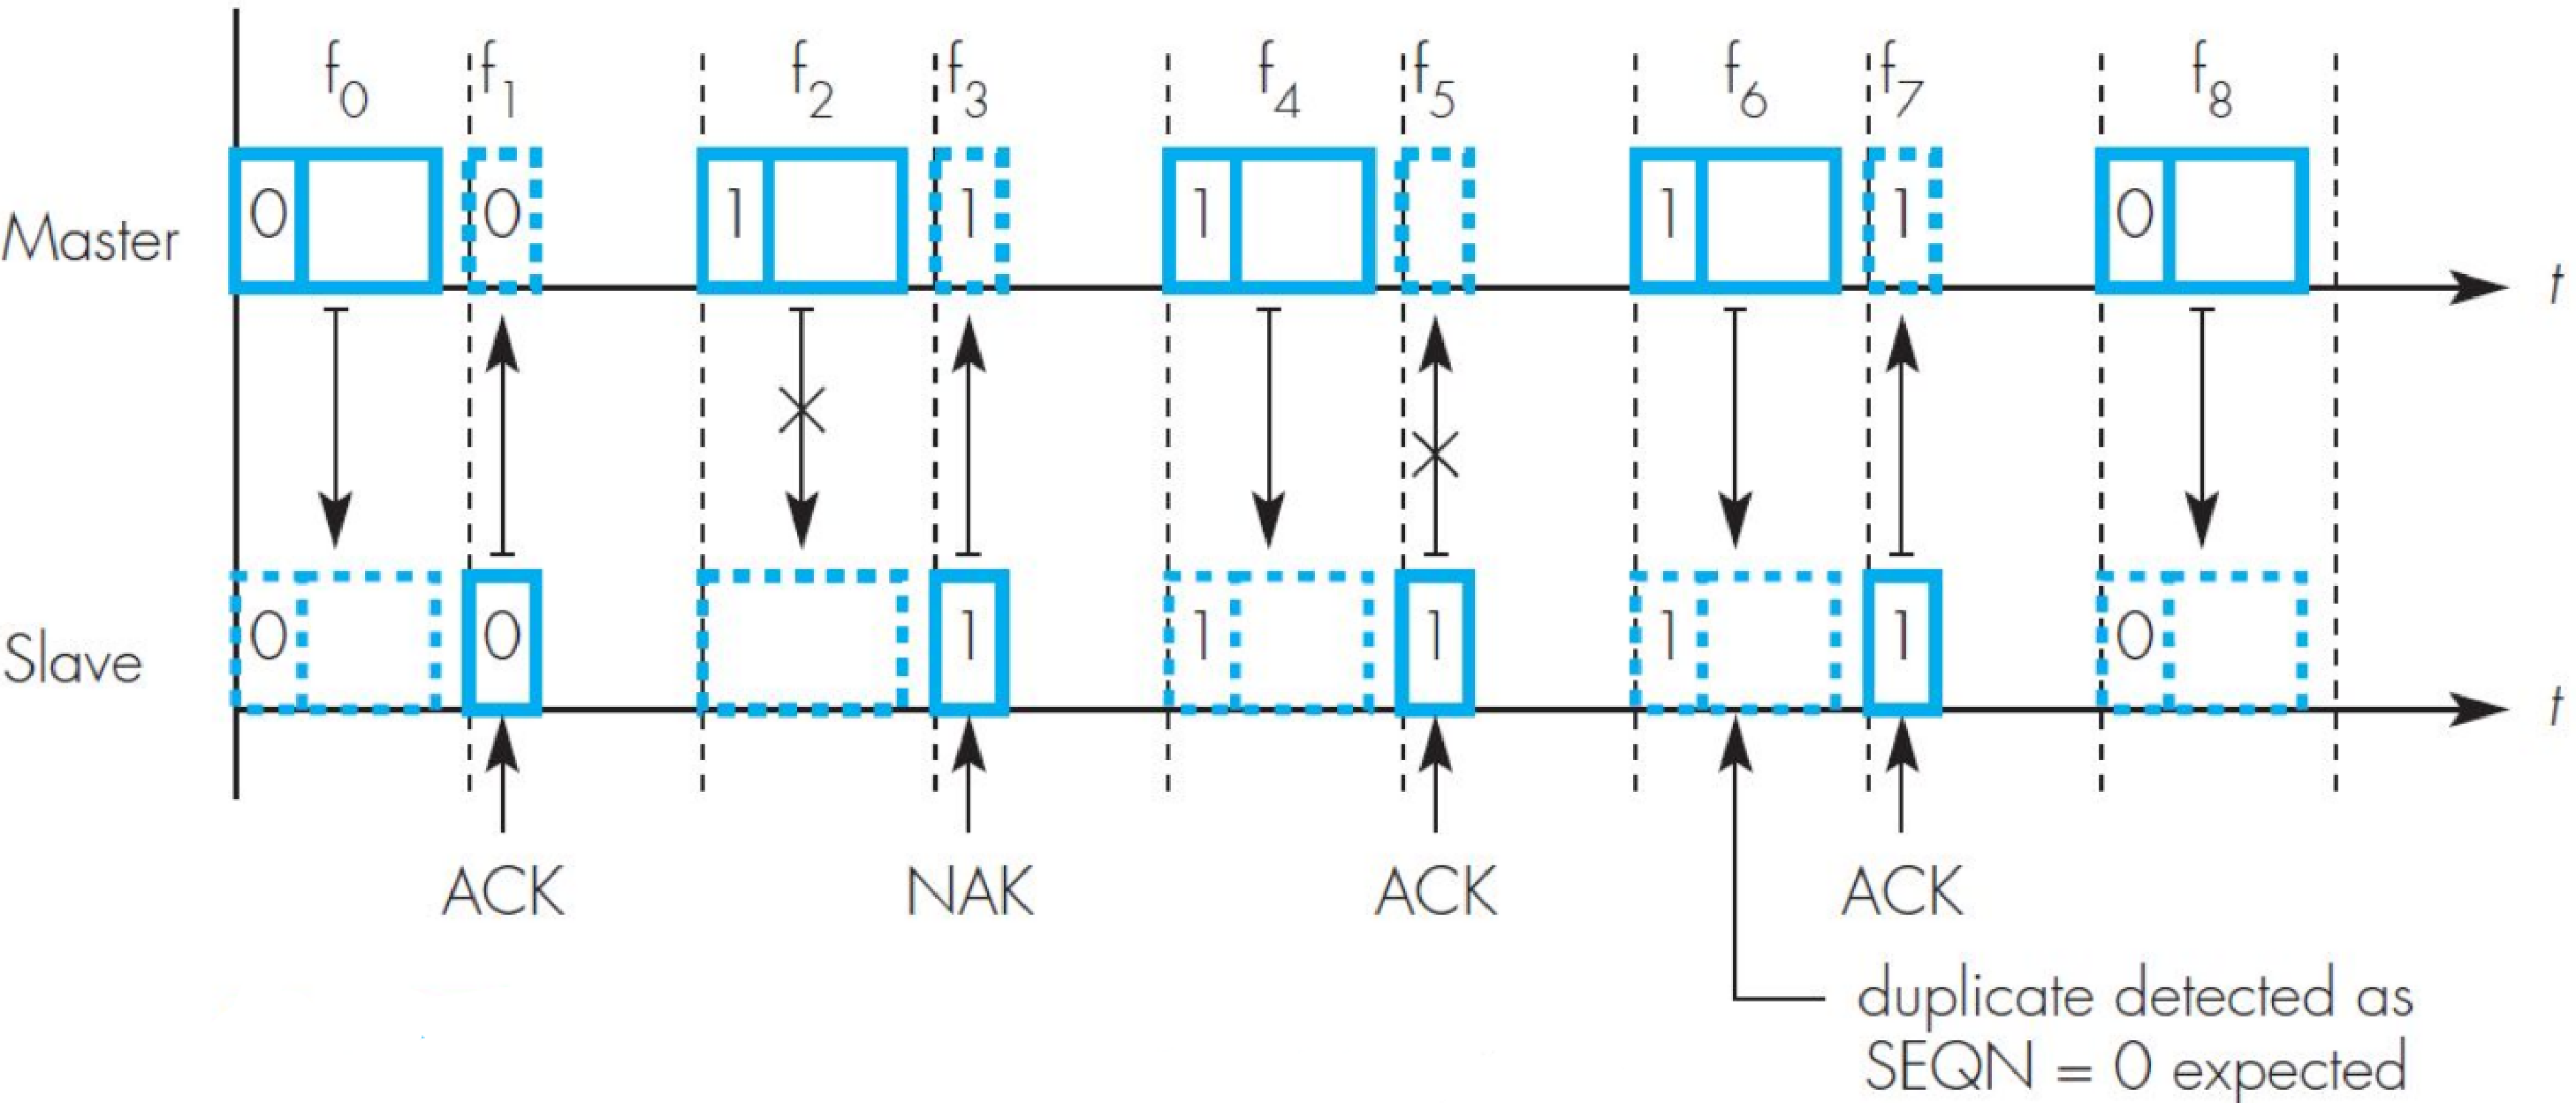
\includegraphics[width=0.9\linewidth]{img/wpan/errorcorr1}
\end{center}

All'interno del quadrato blu si vede il SEQN, mentre ACK/NACK sono indicati al di fuori.\\

Sequenza tipica:
\begin{itemize}
	\item Il master invia un pacchetto con un SEQN $s$
	\item lo slave risponde con un ACK ed un SEQN $s$ (lo stesso)
\end{itemize}

Possibili problemi: 
\begin{itemize}
	\item Lo slave non riceve il pacchetto: invierà un NACK per indicare la mancata ricezione, nello slot successivo deve parlare lo stesso dato che "è il suo turno", sa che ci sarà un SEQN pari a $\neg s$ ma non ha ricevuto nulla e lo indica con il NACK. "Non ho ricevuto e mi aspettavo questo"
	\item Se il master non riceve risposta dallo slave (ACK perso), il pacchetto viene re-inviato, con la possibilità di inviare un duplicato, ma meglio che perdere pacchetti
	\item Lo slave riceve un duplicato e se ne accorge in quanto il SEQN è uguale a quello precedente (il master non ha ricevuto l'ACK, non è cambiato il SEQN, quindi è una ritrasmissione del pacchetto precedente)
\end{itemize}
La rigidità dell'alternanza tra master e slave permette di rendere minimale lo spazio necessario per effettuare il controllo degli errori.\\

\newpage

\subsubsection{Link Manager Protocol}
\paragraph{Transizioni di stato:}
\begin{center}
	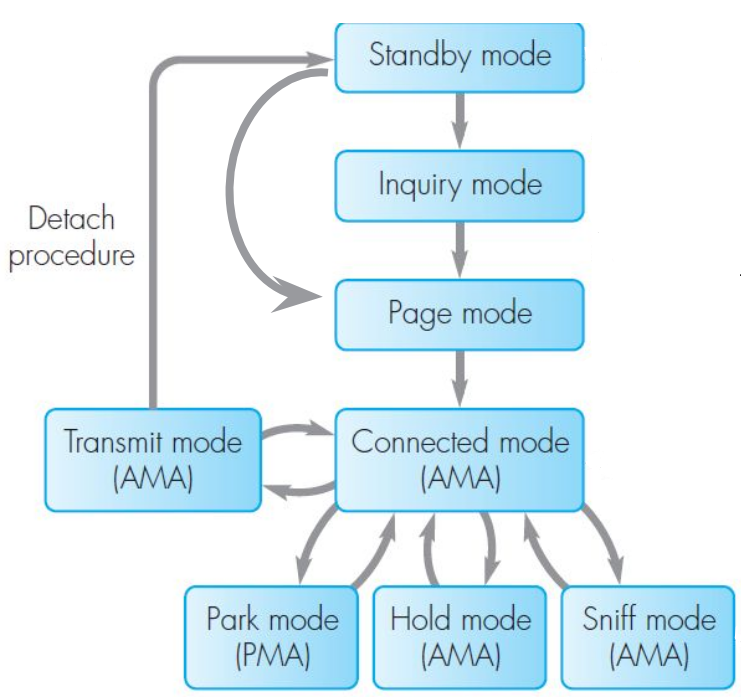
\includegraphics[width=0.55\linewidth]{img/wpan/lmpst}
\end{center}

\paragraph{Standby Mode:} A dispositivo "appena acceso" entra in standby mode, non membro di alcuna piconet, minimo consumo.\\

\paragraph{Enquiry mode:} Periodicamente il master invia 32 messaggi consecutivi usando 32 canali (wake-up channels, la sequenza  è standard). I messaggi contengono un \textbf{IAC packet}. Gli slave periodicamente ascoltano i 32 canali per vedere se qualcuno ha mandato un IAC packet. Tutto questo in modo non coordinato.\\

Ogni dispositivo ascolta per $11,25 ms$, all'inizio di ogni intervallo di $1,28$ o $2,56 s$. Una volta "beccata" una trasmissione del master si aspetta un numero random di slot di tempo (random backoff) prima di trasmettere la risposta (per evitare che più slave che hanno ascoltato quella trasmissione rispondano nello stesso momento). Possiamo farlo dato che adesso l'unica cosa che sappiamo è il clock del master, ricevere un qualsiasi segnale del master permette di sincronizzarsi con la piconet. La risposta contiene il Blouetooth Device Address dello slave e la classe, per indicare il tipo di dispositivo.\\

\newpage

Per finalizzare la connessione mancano le frequenze di hopping: si usano 16 delle 32 frequenze standard, per mandare: Device Access Code DAC, la sequenza di FH e l'Active Member Address AMA dello slave.\\

Lo slave risponde con DAC e ACK, poi può cominciare la comunicazione.
\begin{center}
	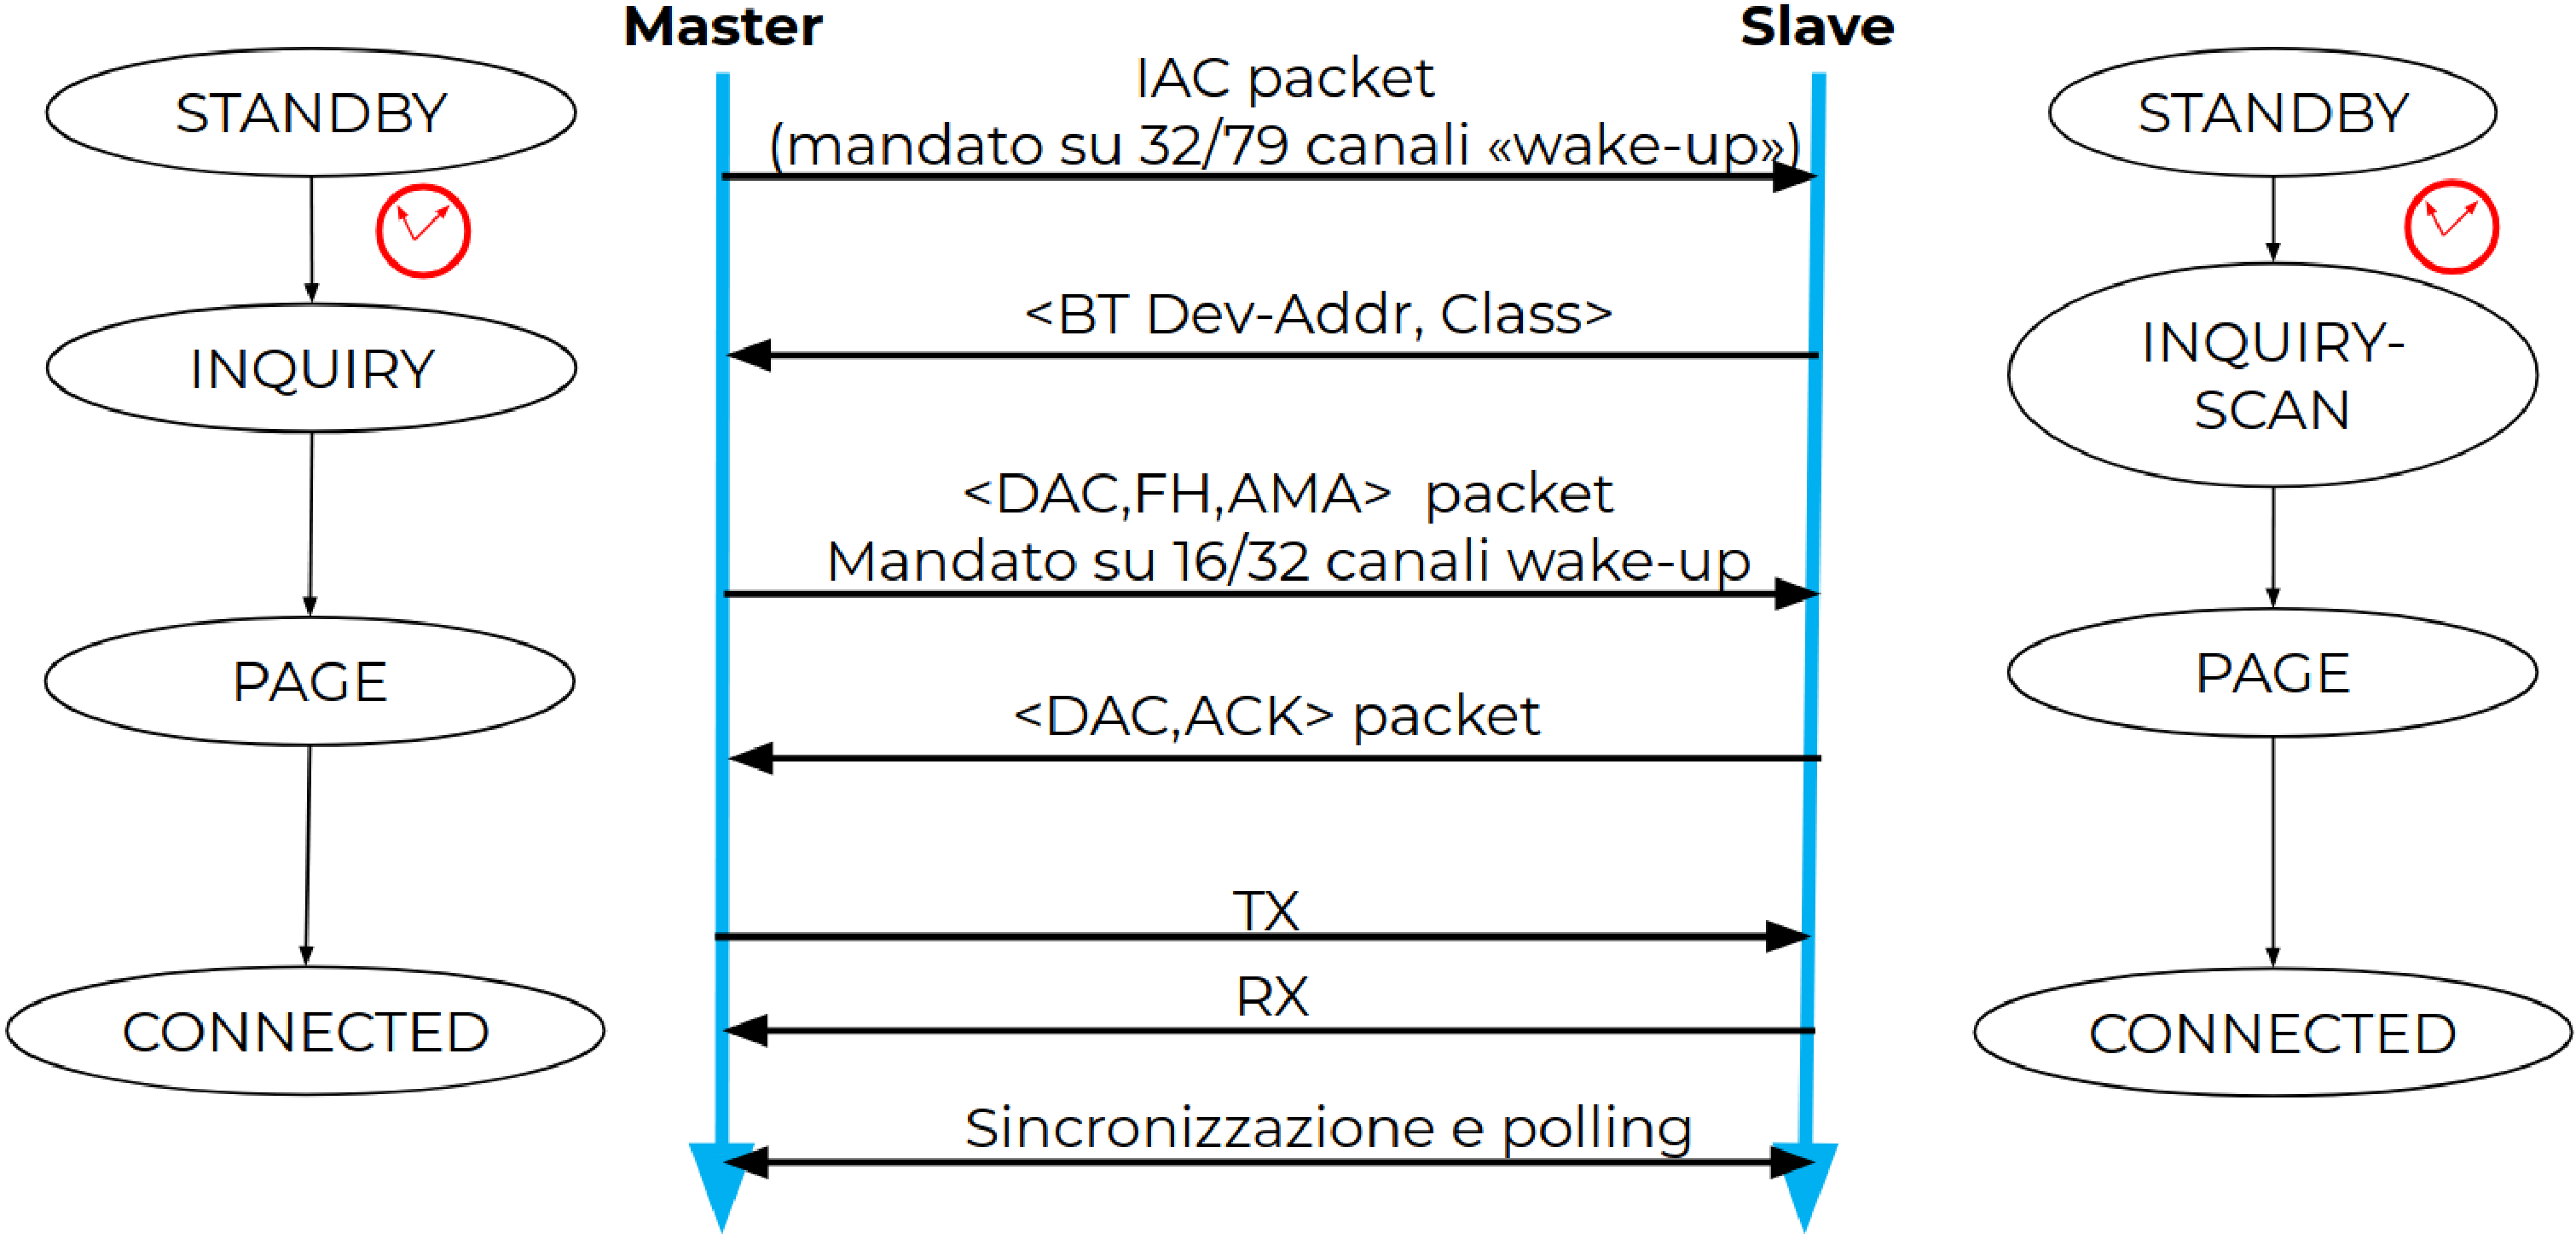
\includegraphics[width=0.95\linewidth]{img/wpan/inquiry1}
\end{center}

%End L6